\section{Zielsetzung}
In dem folgenden Versuch soll das Beugungsbild eines Einzelspalts und eines Doppelspalts aufgenommen und untersucht werden.

\section{Theorie}
\label{sec:Theorie}

Trifft Licht auf Hindernisse z.B. Spalte oder Gitter deren Öffnungen im Vergleich zur Wellenlänge sehr klein sind, wird das Licht gebeugt. An der hinter dem Hindernis stehenden Leinwand o.Ä. wird dann das sogenannte "Beugungsmuster" abbgebildet.

\subsection{Lichtbeugung nach Fresnel und Fraunhofer}
Es existieren zwei grundlegende Versuchsanordnungen, mit denen eine Verteilungsfunktion bestimmt werden kann.
Die Fresnelsche und die Fraunhofersche Lichtbeugung benutzen zunächst den gleichen Versuchsaufbau, einen Spalt mit entsprechenden Abmaßen, die Beugungsebene und ein Schirm und die Beobachtungsebene. Der Unterschied besteht darin in welchem Winkel das Licht auf den Spalt trifft. \\
Bei der Fresnelschen Anordnung befindet sich die Lichtquelle in einem endlichen Abstand zur Beugungsebene, wodurch divergente Lichtbündel entstehen. In Abbildung $\ref{fig:FUF}$ ist zu sehen, dass die divergenten Strahlen unter zwei Brechungswinkeln $\varphi_1 und \varphi_2$ gebrochen werden und dadurch eine Interferenz in Punkt P entsteht.\\

\begin{figure}[H]
  \centering
  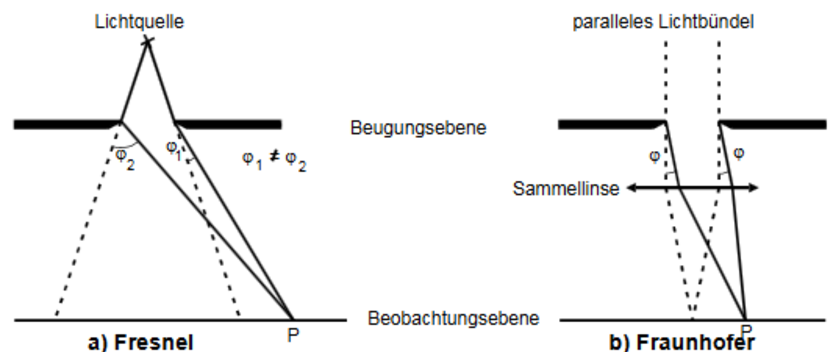
\includegraphics{ressources/FuF.pdf}
  \caption{Darstellung der beiden Anordnungsmöglichkeiten, \cite{skript}.}
  \label{fig:FUF}
\end{figure}

Nach der Fraunhofscher Versuchsanordnung wird die Lichtgequelle im Unendlichen platziert, wodurch die Strahlen parallel auf die Beugungsebene auftreffen. Dadurch werden sie durch den selben Brechungswinkel $\varphi$ gebrochen und erzeugen eine Interferenz im Punkt P. \\
Da die  Fraunhofsche Versuchsanordnung mathematisch einfacher die Beugung von Licht beschreibt wird im folgenden diese Anordnung verwendet.

\subsection{Huygens-Fresnelsches Prinzip}
Mit dem Ansatz, das eine ebene Welle der Form
\begin{align}
  A(z,t) &= A_0 \exp{ \left (i \left(\omega t - \frac{2\pi z}{\lambda} \right) \right) }
  \label{eq:Welle}
\end{align}
sich in Z-Richtung bewegt, besagt das Huygens-Fresnelsche Prinzip, das jeder Punkt einer Wellenfront als Ursprungspunkt einer  Elementarwelle betrachtet werden kann. Somit entstehen beim Durchgang durch den Spalt Kugelwellen, weshalb der Lichtstrahl den Spalt nicht unbeeinflusst passiert. Dadurch werden die parallel einfallenden Lichtstrahlen zu divergenten Lichtstrahlen. Nimmt man nach Abbildung $\ref{fig:ES}$ zwei Lichtstrahlen heraus die um den Winkel $\varphi$ gebeugt wurden, weisen sie aufgrund des Wegunterschiedes $a$ eine Phasendifferenz
\begin{align}
  \delta = \frac{2\pi s}{\lambda} = \frac{2\pi x \sin{(\varphi)}}{\lambda}
  \label{eq:delta}
\end{align}
auf.\\

\begin{figure}[H]
  \centering
  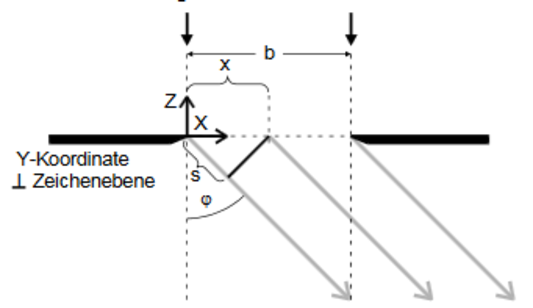
\includegraphics{ressources/ES.pdf}
  \caption{Darstellung der Phasendifferenz zweier einfallender Strahlen, \cite{skript}.}
  \label{fig:ES}
\end{figure}

Um die Amplitude des Beugungsbild in $\varphi$ zu erhalten muss über jeden unter dem Winkel $\varphi$ gebeugten Strahl summiert werden. Durch die obige Phasendifferenz geht die Summe in ein Integral über. Mit der Eulerschen-Formel ergibt sich für die Amplitude
\begin{align}
  B(z,t,\varphi) = A_0 \exp{i \left( \omega t - \frac{2\pi z }{\lambda} \right) } \cdot \exp{ \left( \frac{\pi i b \sin{(\varphi)}}{\lambda} \right) } \cdot \frac{\lambda}{\pi \sin{(\varphi)}} \sin{ \left( \frac{\pi b \sin{(\varphi)}}{\lambda} \right) } \;.
  \label{eq:ES_B_gesamt}
\end{align}
Mit der Abkürzung
\begin{align}
  \eta \coloneqq \frac{\pi b \sin{(\varphi)}}{\lambda}
  \label{eq:eta}
\end{align}
kann die Amplitude durch
\begin{align}
  B(\varphi) = A_0 b \cdot \frac{\sin{(\eta)}}{\eta}
  \label{eq:ES_B}
\end{align}
berechnet werden.
Gleichung $\eqref{eq:ES_B}$ beschreibt eine gerade Funktion mit unendlich vielen Nullstellen, wobei die Maxima und Minima sich immer weiter der Null annähern. Die Funktion ist in Abbildung $\ref{fig:FB}$ für eine beliebige Spaltbreite $b$ und eine beliebige Wellenlänge $\lambda$ dargestellt.

\begin{figure}[H]
  \centering
  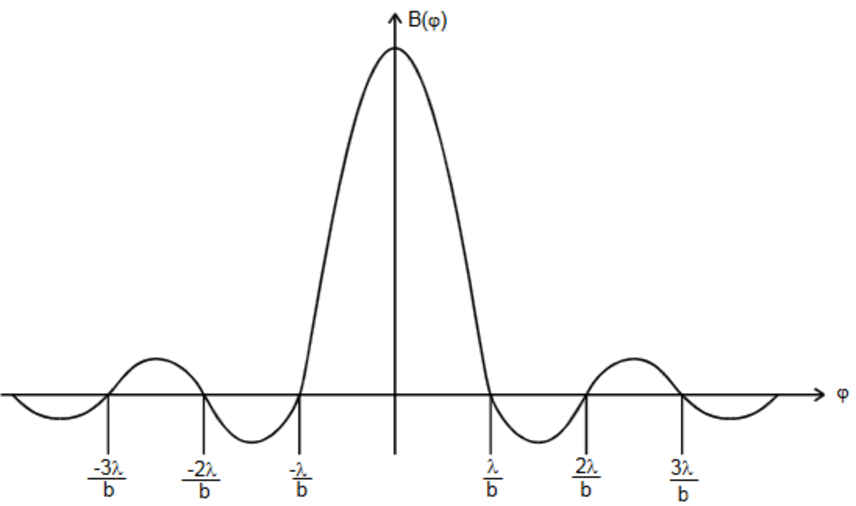
\includegraphics{ressources/Funktion_ES.pdf}
  \caption{Darstellung Amplitudenverteilungsfunktion $B(\varphi)$, \cite{skript}.}
  \label{fig:FB}
\end{figure}

Weiter ergibt sich für die Intensität
\begin{align}
  I(\varphi) \propto B(\varphi)^2 = A_0^2 b^2 \left( \frac{\lambda}{\pi b \sin{(\varphi)}} \right) ^2 \cdot \sin{ \left( \frac{\pi b \sin{(\varphi)}}{\lambda} \right) }^2
  \label{eq:ES_Intensitaet}
\end{align}
Zur Veranschaulichung ist die durch die Quadrierung immer positive Funktion in Abbildung $\ref{fig:Int}$ dargestellt.

\begin{figure}[H]
  \centering
  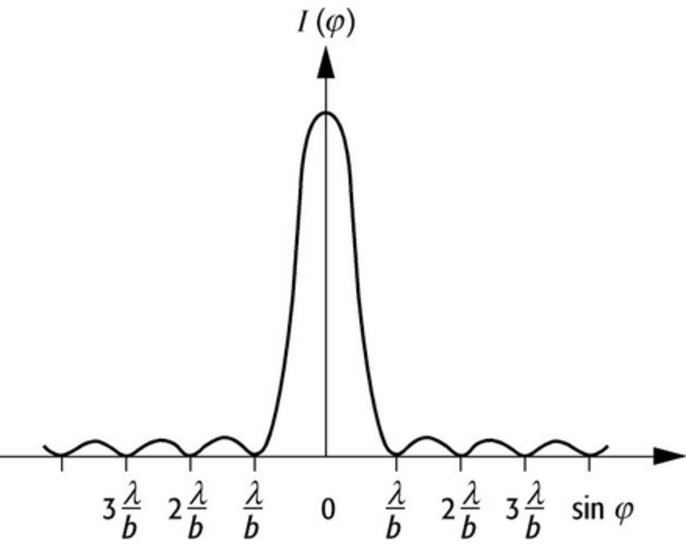
\includegraphics{ressources/Intensitaet.pdf}
  \caption{Darstellung der Intensität $I(\varphi)$, \cite{skript}.}
  \label{fig:Int}
\end{figure}


Nach dem gleichen Prinzip lässt sich die Intensität $I(\varphi)$ für ein in Abbildung $\ref{fig:DS}$ dargestellten Doppelspalt berechnen
\begin{align}
  I(\phi) \propto 4 \cdot \cos{ \left( \frac{\pi s \sin{(\varphi)}}{\lambda} \right) }^2 \cdot \left( \frac{\lambda}{\pi b \sin{(\varphi)}} \right) ^2 \cdot \sin{ \left( \frac{\pi b \sin{(\varphi)}}{\lambda} \right) }^2 \;.
  \label{eq:DS_Intensitaet}
\end{align}

\begin{figure}[H]
  \centering
  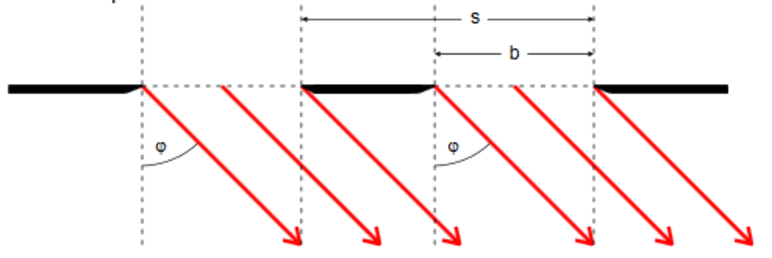
\includegraphics{ressources/DS.pdf}
  \caption{Aufbau eines Doppelspalts, \cite{skript}.}
  \label{fig:DS}
\end{figure}


\subsection{Fourier-Transformation}
Mit der Fouriertransformation der Form
\begin{align}
  g(p)= \int_{-\infty}^{\infty} f(x) \exp{(ixp)} dx
  \label{eq:Fouriertrafo}
\end{align}
lässt sich die Amplitudenverteilungsfunktion $B(\varphi)$ ebenfalls berechnen.\\
Für einen Einzelspalt gilt für die Aperturfunktion 
\begin{align*}
  f(x) &= A_0 \:\:\: \text{für} \: 0 \le x \le b\\
  f(x) &= 0 \:\:\: \text{sonst}\;.
\end{align*}

Somit ergibt sich
\begin{align}
  g(p) = \frac{2A_0}{p} \exp{ \left( \frac{ipb}{2} \right) } \sin{ \left( \frac{pb}{2} \right) }
  \label{eq:fourier}
\end{align}

Im Vergleich von Gleichung  $\eqref{eq:ES_B}$ mit  Gleichung $\eqref{eq:fourier}$ ist zu sehen, das beide Amplitudenverteilungsfunktionen $B(\varphi)$ übereinstimmen.





% 2x2 Plot
% \begin{figure*}
%     \centering
%     \begin{subfigure}[b]{0.475\textwidth}
%         \centering
%         \includegraphics[width=\textwidth]{Abbildungen/Schaltung1.pdf}
%         \caption[]%
%         {{\small Schaltung 1.}}
%         \label{fig:Schaltung1}
%     \end{subfigure}
%     \hfill
%     \begin{subfigure}[b]{0.475\textwidth}
%         \centering
%         \includegraphics[width=\textwidth]{Abbildungen/Schaltung2.pdf}
%         \caption[]%
%         {{\small Schaltung 2.}}
%         \label{fig:Schaltung2}
%     \end{subfigure}
%     \vskip\baselineskip
%     \begin{subfigure}[b]{0.475\textwidth}
%         \centering
%         \includegraphics[width=\textwidth]{Abbildungen/Schaltung4.pdf}    % Zahlen vertauscht ... -.-
%         \caption[]%
%         {{\small Schaltung 3.}}
%         \label{fig:Schaltung3}
%     \end{subfigure}
%     \quad
%     \begin{subfigure}[b]{0.475\textwidth}
%         \centering
%         \includegraphics[width=\textwidth]{Abbildungen/Schaltung3.pdf}
%         \caption[]%
%         {{\small Schaltung 4.}}
%         \label{fig:Schaltung4}
%     \end{subfigure}
%     \caption[]
%     {Ersatzschaltbilder der verschiedenen Teilaufgaben.}
%     \label{fig:Schaltungen}
% \end{figure*}
